\documentclass[12pt,a4paper]{report}

% ============================================================================
% PACKAGES
% ============================================================================
\usepackage[utf8]{inputenc}
\usepackage[T1]{fontenc}
\usepackage{lmodern}
\usepackage[margin=1in]{geometry}
\usepackage{graphicx}
\usepackage{xcolor}
\usepackage{hyperref}
\usepackage{tikz}
\usepackage{longtable}
\usepackage{booktabs}
\usepackage{fancyhdr}
\usepackage{titlesec}
\usepackage{tocloft}
\usepackage{listings}
\usepackage{enumitem}

% TikZ Libraries
\usetikzlibrary{shapes.geometric, arrows.meta, positioning, fit, backgrounds, calc}

% ============================================================================
% COLORS
% ============================================================================
\definecolor{primaryblue}{RGB}{26, 54, 93}
\definecolor{secondaryblue}{RGB}{59, 130, 246}
\definecolor{accentgreen}{RGB}{34, 197, 94}
\definecolor{warningorange}{RGB}{249, 115, 22}
\definecolor{lightgray}{RGB}{243, 244, 246}
\definecolor{darkgray}{RGB}{75, 85, 99}

% ============================================================================
% HYPERREF SETUP
% ============================================================================
\hypersetup{
    colorlinks=true,
    linkcolor=primaryblue,
    filecolor=primaryblue,
    urlcolor=secondaryblue,
    pdftitle={EduX School Management System - Getting Started Guide},
    pdfauthor={EduX Development Team},
}

% ============================================================================
% HEADER/FOOTER
% ============================================================================
\pagestyle{fancy}
\fancyhf{}
\fancyhead[L]{\textcolor{darkgray}{\small EduX School Management System}}
\fancyhead[R]{\textcolor{darkgray}{\small Getting Started Guide}}
\fancyfoot[C]{\textcolor{darkgray}{\thepage}}
\renewcommand{\headrulewidth}{0.4pt}
\renewcommand{\footrulewidth}{0pt}

% ============================================================================
% TITLE FORMATTING
% ============================================================================
\titleformat{\chapter}[display]
  {\normalfont\huge\bfseries\color{primaryblue}}
  {\chaptertitlename\ \thechapter}{20pt}{\Huge}

\titleformat{\section}
  {\normalfont\Large\bfseries\color{primaryblue}}
  {\thesection}{1em}{}

\titleformat{\subsection}
  {\normalfont\large\bfseries\color{secondaryblue}}
  {\thesubsection}{1em}{}

% ============================================================================
% LISTINGS SETUP
% ============================================================================
\lstset{
    backgroundcolor=\color{lightgray},
    basicstyle=\ttfamily\small,
    breaklines=true,
    frame=single,
    rulecolor=\color{darkgray},
}

% ============================================================================
% DOCUMENT
% ============================================================================
\begin{document}

% ----------------------------------------------------------------------------
% TITLE PAGE
% ----------------------------------------------------------------------------
\begin{titlepage}
    \centering
    \vspace*{2cm}
    
    {\Huge\bfseries\textcolor{primaryblue}{EduX}\par}
    \vspace{0.5cm}
    {\Large\textcolor{secondaryblue}{School Management System}\par}
    
    \vspace{2cm}
    
    
\begin{tikzpicture}
        \node[draw=primaryblue, line width=2pt, rounded corners=10pt, 
              minimum width=8cm, minimum height=3cm, fill=lightgray] 
              {\Huge\bfseries\textcolor{primaryblue}{Getting Started Guide}};
    \end{tikzpicture}
    
    \vfill
    
    {\large\textcolor{darkgray}{Version 1.0}\par}
    {\large\textcolor{darkgray}{\today}\par}
    
    \vspace{1cm}
    
    {\textcolor{darkgray}{Offline-First Desktop Application for Educational Institutions}\par}
\end{titlepage}

% ----------------------------------------------------------------------------
% TABLE OF CONTENTS
% ----------------------------------------------------------------------------
\tableofcontents
\newpage

% ============================================================================
% CHAPTER 1: INTRODUCTION
% ============================================================================
\chapter{Introduction}

\section{About EduX}

EduX is a comprehensive, offline-first school management system designed for educational institutions. Built with Flutter for Windows desktop, it provides complete school administration capabilities without requiring internet connectivity.

\subsection{Key Features}

\begin{itemize}[leftmargin=*]
    \item \textbf{Offline-First Operation} -- All data stored locally in SQLite database
    \item \textbf{Student Management} -- Complete student lifecycle from admission to graduation
    \item \textbf{Fee Management} -- Invoicing, payments, concessions, and defaulter tracking
    \item \textbf{Attendance Tracking} -- Daily attendance for students and staff
    \item \textbf{Examination System} -- Exams, marks entry, grading, and report cards
    \item \textbf{Staff Management} -- Employee records, payroll, and leave management
    \item \textbf{Academic Management} -- Classes, sections, subjects, and timetables
    \item \textbf{Reports \& Analytics} -- Comprehensive reporting with PDF/Excel export
    \item \textbf{Backup \& Restore} -- Data safety with automated backups
\end{itemize}

\subsection{User Roles}

EduX supports four user roles with different access levels:

\begin{center}
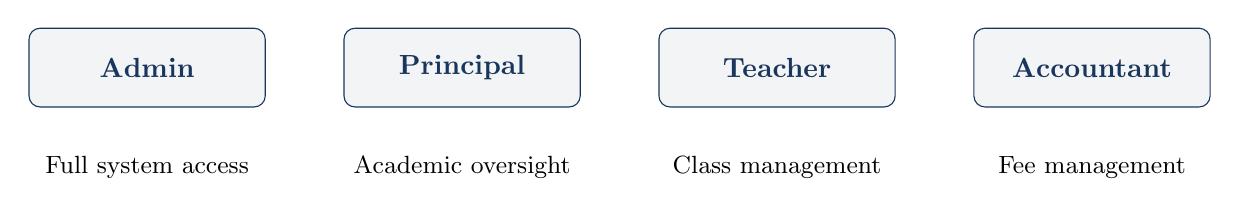
\begin{tikzpicture}[
    role/.style={draw=primaryblue, rounded corners, minimum width=3cm, 
                 minimum height=1cm, fill=lightgray, text=primaryblue, 
                 font=\bfseries},
    arrow/.style={-{Stealth}, thick, primaryblue}
]
    \node[role] (admin) at (0,0) {Admin};
    \node[role] (principal) at (4,0) {Principal};
    \node[role] (teacher) at (8,0) {Teacher};
    \node[role] (accountant) at (12,0) {Accountant};
    
    \node[below=0.5cm of admin, text width=2.8cm, align=center, font=\small] 
        {Full system access};
    \node[below=0.5cm of principal, text width=2.8cm, align=center, font=\small] 
        {Academic oversight};
    \node[below=0.5cm of teacher, text width=2.8cm, align=center, font=\small] 
        {Class management};
    \node[below=0.5cm of accountant, text width=2.8cm, align=center, font=\small] 
        {Fee management};
\end{tikzpicture}
\end{center}

% ============================================================================
% CHAPTER 2: SYSTEM REQUIREMENTS
% ============================================================================
\chapter{System Requirements}

\section{Hardware Requirements}

\begin{longtable}{@{}p{4cm}p{5cm}p{5cm}@{}}
\toprule
\textbf{Component} & \textbf{Minimum} & \textbf{Recommended} \\
\midrule
\endhead
Processor & Intel Core i3 / AMD Ryzen 3 & Intel Core i5 / AMD Ryzen 5 \\
RAM & 4 GB & 8 GB \\
Storage & 500 MB free space & 2 GB free space \\
Display & 1366 × 768 resolution & 1920 × 1080 resolution \\
\bottomrule
\end{longtable}

\section{Software Requirements}

\begin{itemize}[leftmargin=*]
    \item \textbf{Operating System:} Windows 10 (64-bit) or later
    \item \textbf{Visual C++ Redistributable:} 2019 or later (bundled with installer)
\end{itemize}

% ============================================================================
% CHAPTER 3: INSTALLATION
% ============================================================================
\chapter{Installation}

\section{Installation Steps}

\begin{enumerate}[leftmargin=*]
    \item Download the EduX installer from the official source
    \item Run \texttt{EduX\_Setup.exe} as Administrator
    \item Follow the installation wizard prompts
    \item Choose installation directory (default: \texttt{C:\textbackslash Program Files\textbackslash EduX})
    \item Wait for installation to complete
    \item Launch EduX from desktop shortcut or Start Menu
\end{enumerate}

\section{Data Storage Location}

All application data is stored locally:

\begin{lstlisting}
C:\Users\<Username>\AppData\Roaming\EduX\
    |-- edux_database.sqlite    # Main database
    |-- backups\                # Backup files
    |-- exports\                # Exported reports
    |-- logs\                   # Application logs
\end{lstlisting}

% ============================================================================
% CHAPTER 4: FIRST-TIME SETUP
% ============================================================================
\chapter{First-Time Setup}

\section{Setup Wizard}

When launching EduX for the first time, the Setup Wizard will guide you through initial configuration:

\begin{center}
\begin{tikzpicture}[
    node distance=0.8cm,
    step/.style={draw=secondaryblue, rounded corners, minimum width=4cm, 
                 minimum height=1.2cm, fill=lightgray, align=center},
    arrow/.style={-{Stealth}, thick, secondaryblue}
]
    \node[step] (s1) {1. School Information};
    \node[step, below=of s1] (s2) {2. Academic Year Setup};
    \node[step, below=of s2] (s3) {3. Admin Account Creation};
    \node[step, below=of s3] (s4) {4. Classes \& Sections};
    \node[step, below=of s4] (s5) {5. Complete Setup};
    
    \draw[arrow] (s1) -- (s2);
    \draw[arrow] (s2) -- (s3);
    \draw[arrow] (s3) -- (s4);
    \draw[arrow] (s4) -- (s5);
\end{tikzpicture}
\end{center}

\section{School Information}

Enter your school's basic information:

\begin{itemize}[leftmargin=*]
    \item \textbf{School Name} (required)
    \item \textbf{Address, City, State}
    \item \textbf{Phone Number, Email}
    \item \textbf{Principal Name}
    \item \textbf{School Logo} (optional, PNG/JPG format)
\end{itemize}

\section{Academic Year Configuration}

Configure the current academic year:

\begin{itemize}[leftmargin=*]
    \item \textbf{Academic Year Name} (e.g., ``2025-2026'')
    \item \textbf{Start Date} (e.g., April 1, 2025)
    \item \textbf{End Date} (e.g., March 31, 2026)
    \item \textbf{Working Days} (select days school operates)
    \item \textbf{School Timings} (start and end times)
\end{itemize}

\section{Administrator Account}

Create the first administrator account:

\begin{itemize}[leftmargin=*]
    \item \textbf{Username} -- Unique login identifier (minimum 3 characters)
    \item \textbf{Password} -- Strong password (minimum 6 characters)
    \item \textbf{Full Name} -- Administrator's display name
    \item \textbf{Email} (optional) -- For account recovery
\end{itemize}

\textbf{Important:} Store these credentials securely. The admin account has full system access.

% ============================================================================
% CHAPTER 5: NAVIGATION
% ============================================================================
\chapter{Navigation Overview}

\section{Main Interface}

The EduX interface consists of three main areas:

\begin{center}
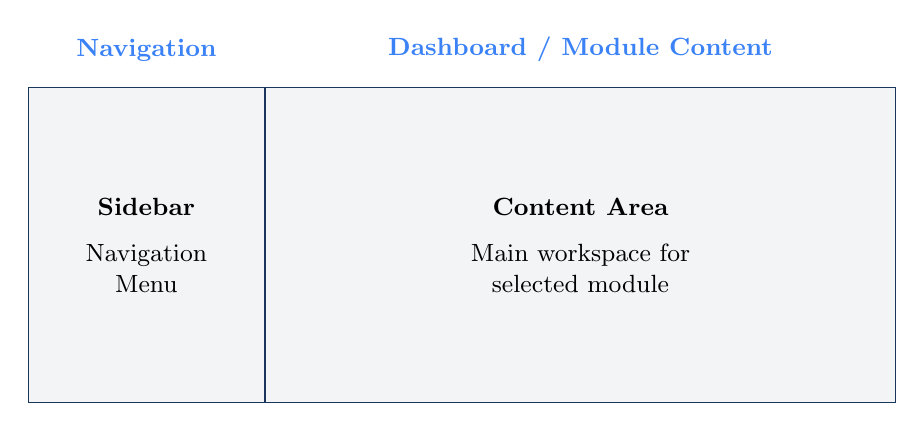
\begin{tikzpicture}[
    area/.style={draw=primaryblue, minimum height=4cm, fill=lightgray, 
                 align=center, font=\small}
]
    % Sidebar
    \node[area, minimum width=3cm] (sidebar) at (0,0) 
        {\textbf{Sidebar}\\[0.2cm] Navigation\\Menu};
    
    % Content Area
    \node[area, minimum width=8cm, right=0cm of sidebar] (content) 
        {\textbf{Content Area}\\[0.2cm] Main workspace for\\selected module};
    
    % Labels
    \node[above=0.2cm of sidebar, font=\bfseries\small, text=secondaryblue] 
        {Navigation};
    \node[above=0.2cm of content, font=\bfseries\small, text=secondaryblue] 
        {Dashboard / Module Content};
\end{tikzpicture}
\end{center}

\section{Navigation Menu}

The sidebar provides access to all modules:

\begin{longtable}{@{}p{3cm}p{10cm}@{}}
\toprule
\textbf{Module} & \textbf{Description} \\
\midrule
\endhead
Dashboard & Overview with statistics, alerts, and quick actions \\
Students & Student registration, profiles, and enrollment \\
Attendance & Daily attendance marking and reports \\
Fees & Invoice generation, payment collection, reports \\
Exams & Exam creation, marks entry, report cards \\
Staff & Employee management, payroll, leave \\
Academics & Classes, sections, subjects, timetable \\
Reports & Analytics and data exports \\
Settings & System configuration and backup \\
\bottomrule
\end{longtable}

% ============================================================================
% CHAPTER 6: QUICK START
% ============================================================================
\chapter{Quick Start Guide}

\section{Recommended First Steps}

After completing setup, follow these steps to get started:

\begin{enumerate}[leftmargin=*]
    \item \textbf{Configure Classes \& Sections}
    \begin{itemize}
        \item Go to \texttt{Academics} $\rightarrow$ \texttt{Classes}
        \item Add all classes (e.g., Playgroup, Nursery, Class 1-10)
        \item Add sections for each class (A, B, C)
    \end{itemize}
    
    \item \textbf{Set Up Subjects}
    \begin{itemize}
        \item Go to \texttt{Academics} $\rightarrow$ \texttt{Subjects}
        \item Add subjects with codes (e.g., ENG, MATH, SCI)
        \item Assign subjects to classes
    \end{itemize}
    
    \item \textbf{Configure Fee Structure}
    \begin{itemize}
        \item Go to \texttt{Fees} $\rightarrow$ \texttt{Fee Types}
        \item Create fee types (Tuition, Transport, etc.)
        \item Set class-wise fee structures
    \end{itemize}
    
    \item \textbf{Register Students}
    \begin{itemize}
        \item Go to \texttt{Students} $\rightarrow$ \texttt{Add Student}
        \item Enter student and guardian information
        \item Enroll in appropriate class/section
    \end{itemize}
    
    \item \textbf{Create User Accounts}
    \begin{itemize}
        \item Go to \texttt{Settings} $\rightarrow$ \texttt{Users}
        \item Create accounts for teachers and staff
        \item Assign appropriate roles
    \end{itemize}
\end{enumerate}

\section{Daily Operations}

\begin{center}
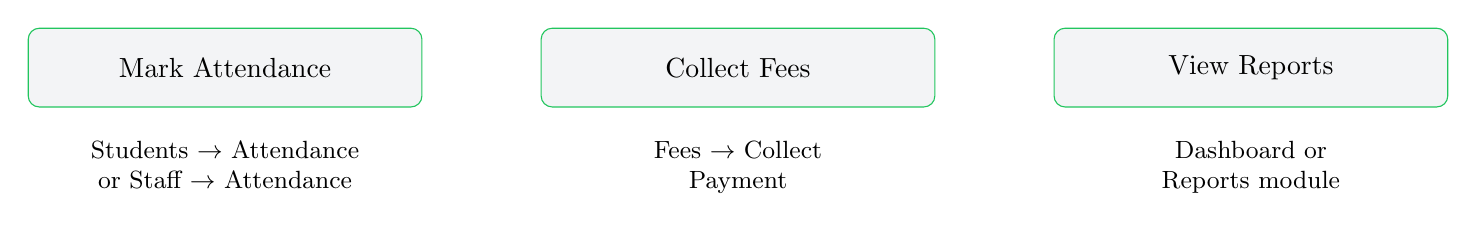
\begin{tikzpicture}[
    node distance=1.5cm,
    task/.style={draw=accentgreen, rounded corners, minimum width=5cm, 
                 minimum height=1cm, fill=lightgray, align=center}
]
    \node[task] (t1) {Mark Attendance};
    \node[task, right=of t1] (t2) {Collect Fees};
    \node[task, right=of t2] (t3) {View Reports};
    
    \node[below=0.3cm of t1, font=\small, text width=4.5cm, align=center] 
        {Students $\rightarrow$ Attendance\\or Staff $\rightarrow$ Attendance};
    \node[below=0.3cm of t2, font=\small, text width=4.5cm, align=center] 
        {Fees $\rightarrow$ Collect\\Payment};
    \node[below=0.3cm of t3, font=\small, text width=4.5cm, align=center] 
        {Dashboard or\\Reports module};
\end{tikzpicture}
\end{center}

% ============================================================================
% CHAPTER 7: KEYBOARD SHORTCUTS
% ============================================================================
\chapter{Keyboard Shortcuts}

\section{Global Shortcuts}

\begin{longtable}{@{}p{4cm}p{9cm}@{}}
\toprule
\textbf{Shortcut} & \textbf{Action} \\
\midrule
\endhead
\texttt{Ctrl + D} & Go to Dashboard \\
\texttt{Ctrl + S} & Go to Students \\
\texttt{Ctrl + A} & Go to Attendance \\
\texttt{Ctrl + F} & Go to Fees \\
\texttt{Ctrl + E} & Go to Exams \\
\texttt{Ctrl + T} & Go to Staff \\
\texttt{Ctrl + R} & Go to Reports \\
\texttt{Ctrl + ,} & Open Settings \\
\texttt{Ctrl + B} & Create Backup \\
\texttt{Ctrl + Q} & Logout \\
\texttt{Escape} & Close dialog / Go back \\
\bottomrule
\end{longtable}

% ============================================================================
% CHAPTER 8: GETTING HELP
% ============================================================================
\chapter{Getting Help}

\section{In-App Help}

\begin{itemize}[leftmargin=*]
    \item \textbf{Tooltips} -- Hover over interface elements for descriptions
    \item \textbf{Empty States} -- Helpful guidance when sections have no data
    \item \textbf{Validation Messages} -- Clear error messages for form inputs
\end{itemize}

\section{Data Backup}

\textbf{Important:} Regularly backup your data to prevent data loss.

\begin{enumerate}[leftmargin=*]
    \item Go to \texttt{Settings} $\rightarrow$ \texttt{Backup}
    \item Click \texttt{Create Backup}
    \item Choose destination (local folder or external drive)
    \item Confirm backup completion
\end{enumerate}

\textbf{Tip:} Enable automatic backups in Settings for daily protection.

\end{document}
